%
% relazione_es5.tex
%
% Copyright (C) 2016 frnmst (Franco Masotti) <franco.masotti@student.unife.it>
%                    dannylessio (Danny Lessio)
%
% This file is part of networks-lab.
%
% networks-lab is free software: you can redistribute it and/or modify
% it under the terms of the GNU General Public License as published by
% the Free Software Foundation, either version 3 of the License, or
% (at your option) any later version.
%
% networks-lab is distributed in the hope that it will be useful,
% but WITHOUT ANY WARRANTY; without even the implied warranty of
% MERCHANTABILITY or FITNESS FOR A PARTICULAR PURPOSE.  See the
% GNU General Public License for more details.
%
% You should have received a copy of the GNU General Public License
% along with networks-lab.  If not, see <http://www.gnu.org/licenses/>.
%


\makeatletter
\def\blfootnote{\xdef\@thefnmark{}\@footnotetext}
\makeatother

\documentclass[9pt, a4paper, oneside]{article}
\usepackage[a4paper]{geometry}
\usepackage{graphicx} % pictures
\usepackage{float} % used for H option in pictures                        
\usepackage{setspace} % packets
\usepackage{listings}
\singlespacing % interlinea singolo
\title{Relazione esercitazione 6 Laboratorio di reti\newline
Configurazione di un router CISCO}
\author{Franco Masotti \and Danny Lessio}
\date{June 8, 2015}
\begin{document}
	\maketitle
	\tableofcontents
	\newpage
    \footnotetext{networks-lab  Copyright (C) 2016  frnmst (Franco Masotti), 
dannylessio (Danny Lessio).  This document comes with ABSOLUTELY NO WARRANTY.
This is free software, and you are welcome to redistribute it 
under certain conditions; see LICENSE file for details.}
	\part{Consegna}
			\par
				Questa esercitazione consiste nella 
				configurazione di un router CISCO in modo 
				effetuare il recovery della password e 
				dell'immagine del sistema. Inoltre abbiamo 
				abilitato le rotte statiche e poi quelle 
				quelle dinamiche (con vari algoritmi di 
				routing).
			\par
				Di seguito \'e rappresentato lo schema dei 
				collegamenti tra le seriali di tutti i router:
				\begin{figure}[H]
					\centering
					\caption{Connessioni seriali}
					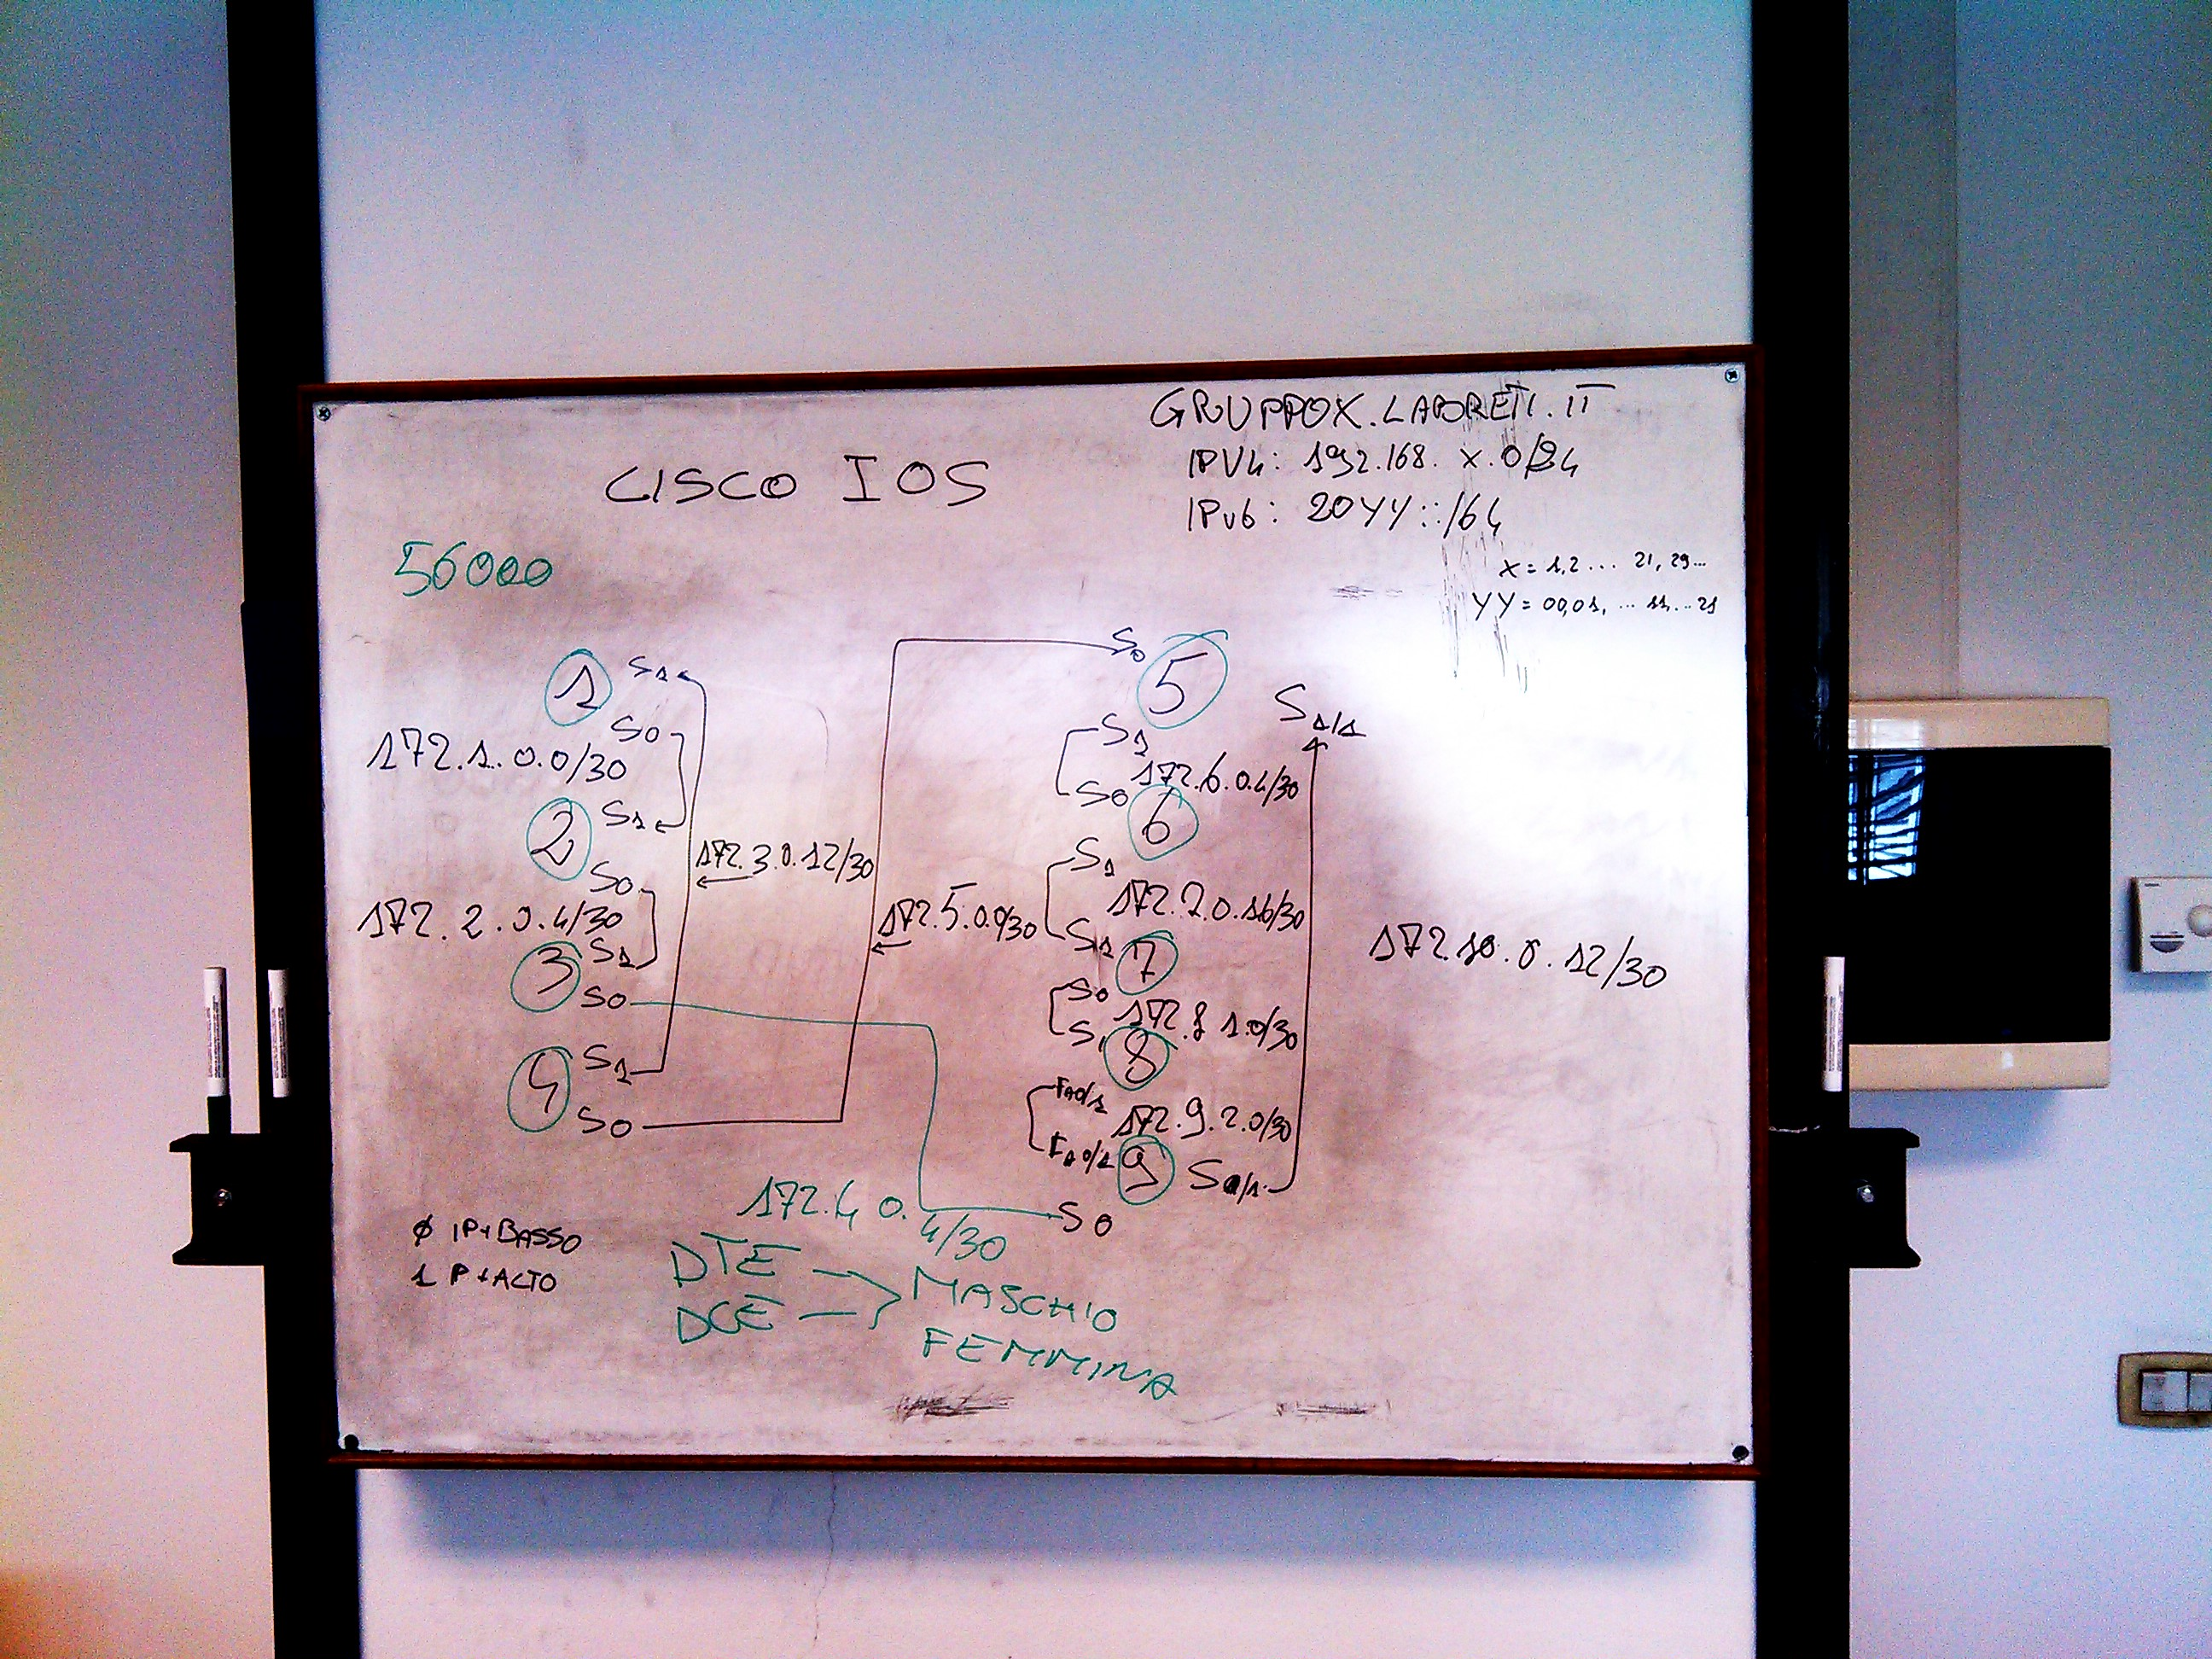
\includegraphics[scale=0.16]{../source/schema_connessioni.jpg}
				\end{figure}
		\newpage
	\part{Configurazione del router}
		\section{Collegamento al router}
			\par
				Al contrario degli switch i nostri router si 
				trovano in una postazione remota. Il 
				collegamento in seriale non \'e quindi pi\'u 
				possibile. In questo caso ci colleghiamo ad un 
				gateway attraverso ethernet con \texttt{telnet}:
				\begin{verbatim}
telnet 192.168.0.100 7002
				\end{verbatim}
				dove la porta 7002 corrisponde al router del 
				nostro gruppo.Abbiamo inserito il nostro 
				username e 
				password\footnote{\texttt{labreti2}}.
			\par 
				Successivamente abbiamo configurato il router 
				allo stesso modo dello switch (escludendo 
				ovviamente la parte delle VLAN che qui non \'e 
				presente) e abbiamo abilitato il telnet.
		\section{Ripristino della password}
				Dopo aver salvato la nostra nuova 
				configurazione sul 
				computer\footnote{\texttt{copy 
				running-config tftp:}} abbiamo salvato anche
				l'immagine del sistema\footnote{\texttt{copy 
				c2600-adventerprisek9-mz.124-16b.bin tftp:}}.
				A questo punto abbiamo settato un valore nel 
				registro di sistema in modo che al riavvio del 
				router, questo ignori la configurazione 
				precedentemente salvata in nvram 
				(\texttt{nvram:/startup-config}):
				\begin{verbatim}
enable
configure terminal
confreg 0x0
end
				\end{verbatim}
				Riavviamo il router con \texttt{reload}
				. Abbiamo poi copiato la vecchia configurazione 
				ed impostato la nuova password:
				\begin{verbatim}
confreg 0x2142
copy startup-config running-config
configure terminal
enable password labreti				
				\end{verbatim}
				Infine abbiamo settato il valore del registro 
				con quello originale:
				\begin{verbatim}
confreg 0x2102
				\end{verbatim}
				
		\section{Ripristino dell'immagine}
			\par
				Se l'immagine del sistema operativo \'e 
				corrotta, allora \'e possibile ripristinarla.
				Ricordandoci che abbiamo salvato l'immagine 
				precedentemente (assumendo che quella non 
				abbia problemi) per prima cosa dobbiamo 
				cancellare l'immagine corrente:
				\begin{verbatim}
enable
cd flash:/
delete c2600-adventerprisek9-mz.124-16b.bin
				\end{verbatim}
			\par
				Adesso riavviamo il router con \texttt{reload}.
				Una volta riavviato il router, noteremo che 
				questo \'e entrato in recovery mode. Per 
				rispristinare l'immagine bisogna assegnare 
				manualmente le informazioni per l'interfaccia 
				ethernet\footnote{Avendo avuto problemi con il 
				server tftp sul computer abbiamo usato quello 
				interno della rete sia per salvare l'immagine 
				sia per effettuare il ripristino.}. Per visualizzare le variabili settate prima di lanciare il comando \texttt{tftpdnld} \'e possibile 
				lanciare il comando \texttt{set}.:
				\begin{verbatim}
IP_ADDRESS=192.168.0.101
IP_SUBNET_MASK=255.255.255.0
DEFAULT_GATEWAY=192.168.0.101
TFTP_SERVER=192.168.0.100
TFTP_FILE=c2600-adventerprisek9-mz.124-16b.bin
				\end{verbatim}
				Abbiamo poi lanciato il comando 
				\texttt{tftpdnld} e abbiamo risposto \texttt{y} 
				a tutte le domande. Per salvare le variabili \texttt{ROMmon} in memoria non volatile \texttt{NVRAM} abbiamo lanciato il comando \texttt{sync}. Infine abbiamo 
				cancellato la nostra configurazione per i 
				prossimi gruppi:
				\begin{verbatim}
delete nvram:/startup-config
reload
				\end{verbatim}				
		\section{Access lists}
			\par
				La parte successiva dell'esercitazione consiste 
				nell'applicazione di access list per inibire 
				l'accesso all'interfaccia amministrativa telnet 
				a certe reti ed host piuttosto che altri.
				Abbiamo provato due casi differenti.
			\par
				Per applicare le access list:
				\begin{verbatim}
enable
configure terminal
ip access-list extended VTY_ACCESS
				\end{verbatim}
			\par
				Il primo caso consiste nel permettere l'accesso 
				a tutti gli host della sottorete escluso il 
				computer corrente:
				\begin{verbatim}
10 permit tcp 192.168.2.0 0.0.0.255 any eq telnet
20 deny tcp host 192.168.2.1 any eq telnet
				\end{verbatim}
			\par
				Il secondo caso invece permette l'accesso solo 
				dal ciomputer corrente mentre inibisce 
				l'accesso da tutti gli altri host.
				\begin{verbatim}
10 permit tcp host 192.168.2.1 any eq telnet
20 deny tcp 192.168.2.0 0.0.0.255 any eq telnet
				\end{verbatim}
			\par
				Per testare queste configurazioni abbiamo 
				usato i due indirizzi \texttt{192.168.2.1} e 
				\texttt{192.168.2.2} a seconda dei casi.
		\section{Configurazioni delle interfaccie seriali}
			\par
				Una delle parti critiche nella fase di setup di ogni router \'e la selezione dei cavi seriali. I device che comunicano attraverso interfaccia seriale vengono suddivisi in due categorie: DCE e DTE. I primi forniscono il segnale di clock per permettere la comunicazione all'interno del bus. Il DTE pu\'o essere visto come "maschio" mentre il DCE viene visto come "femmina".
				\par
				Il router a noi affidato era provvisto di due DTE, non abbiamo dunque avuto bisogno di assegnare il clockrate ed il bandwidth.
				\par
				I router sono collegati tra di loro attraverso queste 
				interfacce seriali. Per poter effettuare il 
				collegamento fra il nostro router e quelli 
				adiacenti (vedi schema connessioni) \'e necessario 
				assegnare due indirizi di sottoreti 
				rispettivamente alle due interfacce.
				Per convenzione la maschera della sottorete 
				\'e \texttt{/30}, quindi abbiamo solo 4 indirizzi 
				disponibili di cui uno usato per identificare 
				la sottorete (\texttt{172.1.0.0} ed 
				\texttt{172.2.0.4}) ed uno per il broadcast 
				(\texttt{172.1.0.3} ed \texttt{172.2.0.7}). 
				Lo scopo finale \'e quello di poter pingare i 
				router adiacenti\footnote{Nel nostro caso il 
				gruppo 1 ed il gruppo 3.}. Come da schema 
				abbiamo assegnato l'indrizzo \texttt{172.2.0.5}
				alla \texttt{Serial0/0} e \texttt{172.1.0.1}
				alla \texttt{Serial0/1}:
				\begin{verbatim}

enable
configure terminal
interface Serial0/0
ip address 172.2.0.5 255.255.255.252
no shut
exit
configure terminal
interface Serial0/1
ip address 172.1.0.1 255.255.255.252
no shut

				\end{verbatim}
				\par 
				A questo punto, \'e stato possibile pingare i router vicini (gruppo1 e gruppo3) attraverso interfaccia seriale con successo:
				\begin{verbatim}
				ping 172.1.0.2
				ping 172.2.0.6
				\end{verbatim}
		\section{Rotte statiche}
			\par
			 L'instradamento deve avvenire dal \texttt{gruppo1} verso il \texttt{gruppo9}. Dev'essere possibile pingare tutti i 9 router della rete interna. 
			 Nella nostra situazione, seguendo lo schema, abbiamo settato la tabella di routing indirizzando i pacchetti relativi alla sottorete 192.168.1.0 al router numero 1, mentre tutti gli altri vengono gestiti dal router numero 3: 
				\begin{verbatim}
ip route 192.168.1.0 255.255.255.0 172.1.0.2 
ip route 0.0.0.0 0.0.0.0 172.2.0.6 
				\end{verbatim}
				A questo punto \'e stato possibile raggiungere 
				ogni altro router a partire dal nostro.
				\par
				Ovviamente, agendo sulle nostre singole macchine ed impostando il nostro router (192.168.2.100) come default gateway \'e stato possibile raggiungere le macchine degli altri gruppi collegate ai rimanenti 8 router locali.
		\section{Rotte dinamiche}
			\par
				Abbiamo applicato tre algoritmi di 
				routing sia di tipo distance vector, sia di 
				tipo link state\footnote{Il comando network di ogni protocollo va applicato per tutte e 3 le interfacce. vedi listato OSPF.}:
				\begin{itemize}
					\item
						RIPv2
						\begin{itemize}
							\item
								\'E di tipo 
								distance 
								vector quindi impiega il numero di hop come metrica. RIP evita i routing loop adottando un limite massimo di hop dalla sorgente verso la destinazione. Il numero massimo di hop consentito \'e 15. Questo numero di hop limita in ogni caso il diametro della rete consentito da RIP. Un numero di hop equivalente a 16 viene considerato come metrica infinita per indicare le rotte inaccessibili che non verranno installate in tabella di routing. Questa versione "v2" include il trasporto di informazioni nella maschera di sottorete. Ecco i comandi per abilitarlo:
								\begin{verbatim}
									router rip
									version 2
									network ip-address mask
								\end{verbatim}
						\end{itemize}
					\item
						OSPF
						\begin{itemize}
							\item
								\'E di tipo 
								link state, 
								cio\'e i link 
								sono scelti in 
								base alle 
								condizioni 
								della rete. 
								OSPF non \'e un 
								protocollo 
								proprietario.
								Aggiunge propriet\'a aggiuntive
                            	rispetto ai protocolli di tipo 								
                                link state quali il bilanciamento del carico, 
                                aggiunge un grado di gerarchia nei domini ed 
                                implementa l'autenticazione dei messaggi.
								Ecco i comandi per abilitarlo:								
								\begin{verbatim}
									router ospf process_id
									network ip_address mask area area_id
								\end{verbatim}
						\end{itemize}
					\item
						EIGRP
						\begin{itemize}
							\item
								Il protocollo 
								propritario 
								della CISCO ha 
								gli aspetti 
								migliori di un 
								protocollo link 
								state e 
								distance 
								vector.
								Ecco i comandi per abilitarlo:
								\begin{verbatim}
									router eigrp autonomous-system
									network network-number
									
								\end{verbatim}
						\end{itemize}
				\end{itemize}
		\newpage	
	\part{Listati}	
		 \par		
		 Abbiamo inserito la sola configurazione del protocollo OSPF, le altre due configurazioni mancanti sono quasi identiche in quanto cambiano solo le informazioni relative al protocollo.		
		 \section{\texttt{running-config} OSPF}
			\par
				\texttt{running-config}
			\par
				File di configurazione principale del router 
				configurato per il routing OSPF. Da notare 
				\texttt{area 12} che deve essere uguale per 
				tutti i router.
			\texttt{\lstinputlisting[breaklines]{../source/running-config-ospf}}
			\newpage
\end{document}
				
